% *********************************************************************
% © 2021 Jeremy Sylvestre
%
% Permission is granted to copy, distribute and/or modify this document
% under the terms of the GNU Free Documentation License, Version 1.3 or
% any later version published by the Free Software Foundation; with no
% Invariant Sections, no Front-Cover Texts, and no Back-Cover Texts. A
% copy of the license is included in the appendix entitled “GNU Free
% Documentation License” that appears in the output document of this
% PreTeXt source code. All trademarks™ are the registered® marks of
% their respective owners.
%
% *********************************************************************

\newcommand*{\xmin}{-0.25}
\newcommand*{\xmax}{4}
\newcommand*{\ymin}{-0.5}
\newcommand*{\ymax}{7}

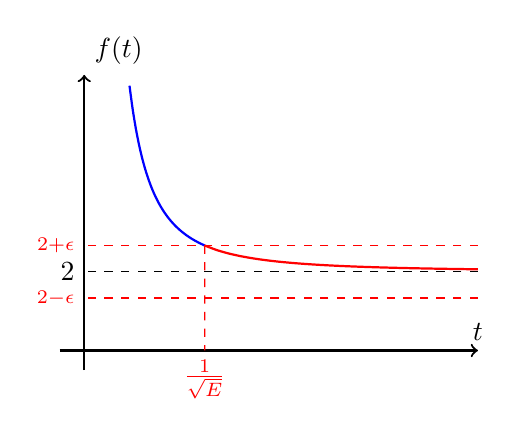
\begin{tikzpicture}
[
	closedpt/.style={circle,draw,fill,inner sep=0pt,minimum size=4pt},
	openpt/.style={circle,draw,inner sep=0pt,minimum size=4pt},
	yscale=0.5,
	xscale=1.25
]

	% axes
	\draw[->,thick] (\xmin,0) -- (\xmax,0) node[above] {$t$};
	\draw[->,thick] (0,\ymin) -- (0,\ymax) node[above right] {$f(t)$};

	% graph
	\draw[thick, blue, domain=0.46:1.225, smooth] plot (\x,{2 + 1 / (\x * \x)});
	\draw[thick, red, domain=1.225:\xmax, smooth] plot (\x,{2 + 1 / (\x * \x)});
	\draw[dashed] (\xmax,2) -- (0,2) node[left] {$2$};
	\draw[dashed,red] (\xmax,1.333) -- (0,1.333) node[left] {$\scriptstyle 2 - \epsilon$};
	\draw[dashed,red] (\xmax,2.666) -- (0,2.666) node[left] {$\scriptstyle 2 + \epsilon$};
	\draw[dashed,red] (1.225,2.666) -- (1.224,0) node[below] {$\frac{1}{\sqrt{E}}$};

\end{tikzpicture}
